%%% LaTeX Template: Two column article
%%%
%%% Source: http://www.howtotex.com/
%%% Feel free to distribute this template, but please keep to referal to http://www.howtotex.com/ here.
%%% Date: February 2011

%%% Preamble
\documentclass[	DIV=calc,%
							paper=a4,%
							fontsize=12pt,%
							onecolumn]{scrartcl}	 					% KOMA-article class

\usepackage{lipsum}													% Package to create dummy text
\usepackage[english]{babel}										% English language/hyphenation
\usepackage[protrusion=true,expansion=true]{microtype}				% Better typography
\usepackage{amsmath,amsfonts,amsthm}					% Math packages
\usepackage[pdftex]{graphicx}									% Enable pdflatex
\usepackage[svgnames]{xcolor}									% Enabling colors by their 'svgnames'
\usepackage[hang, small,labelfont=bf,up,textfont=it,up]{caption}	% Custom captions under/above floats
\usepackage{epstopdf}												% Converts .eps to .pdf
\usepackage{subfig}													% Subfigures
\usepackage{booktabs}												% Nicer tables
\usepackage{fix-cm}													% Custom fontsizes
\usepackage[utf8]{inputenc}
\usepackage[top=2.5cm, bottom=2.5cm, left=2.5cm, right=2.5cm]{geometry}
\usepackage[ddmmyyyy]{datetime}
\usepackage{float}
\addto\captionsenglish{%
	\renewcommand\tablename{Tabela}
	\renewcommand\figurename{Figura}
} 
 

 
%%% Custom sectioning (sectsty package)
\usepackage{sectsty}													% Custom sectioning (see below)
\allsectionsfont{%															% Change font of al section commands
	\usefont{OT1}{phv}{b}{n}%										% bch-b-n: CharterBT-Bold font
	}

\sectionfont{%																% Change font of \section command
	\usefont{OT1}{phv}{b}{n}%										% bch-b-n: CharterBT-Bold font
	}



%%% Headers and footers
\usepackage{fancyhdr}												% Needed to define custom headers/footers
	\pagestyle{fancy}														% Enabling the custom headers/footers
\usepackage{lastpage}	

% Header (empty)
\lhead{}
\chead{}
\rhead{}
% Footer (you may change this to your own needs)

%% ====================================
%% ====================================
%% mude o rodape  do projeto
%% ====================================
%% ====================================

\lfoot{\footnotesize \texttt{Cabeamento estruturado} \textbullet ~Projeto - 2017}


\cfoot{}
\rfoot{\footnotesize página \thepage\ de \pageref{LastPage}}	% "Page 1 of 2"
\renewcommand{\headrulewidth}{0.0pt}
\renewcommand{\footrulewidth}{0.4pt}



%%% Creating an initial of the very first character of the content
\usepackage{lettrine}
\newcommand{\initial}[1]{%
     \lettrine[lines=3,lhang=0.3,nindent=0em]{
     				\color{DarkGoldenrod}
     				{\textsf{#1}}}{}}



%%% Title, author and date metadata
\usepackage{titling}															% For custom titles

\newcommand{\HorRule}{\color{DarkGoldenrod}%			% Creating a horizontal rule
									  	\rule{\linewidth}{1pt}%
										}

\pretitle{\vspace{-70pt} \begin{flushleft} \HorRule 
				\fontsize{40}{40} \usefont{OT1}{phv}{b}{n} \color{DarkRed} \selectfont 
				}

%% ====================================
%% ====================================
%% mude o titulo  do projeto
%% ====================================
%% ====================================

\title{Projeto de cabeamento estruturado}					% Title of your article goes here

%% ====================================



\posttitle{\par\end{flushleft}\vskip 0.5em}

\preauthor{\begin{flushleft}
					\large \lineskip 0.5em \usefont{OT1}{phv}{b}{sl} \color{DarkRed}}
\author{Marcos Santana Viana}  	% Author name goes here


\postauthor{\footnotesize \usefont{OT1}{phv}{m}{sl} \color{Black} 
					\\Universidade Tecnológica Federal do Paraná - Câmpus Cornélio Procópio 								% Institution of author
					\par\end{flushleft}\HorRule}

\date{}																				% No date




%%% Begin document
\begin{document}
\maketitle
\thispagestyle{fancy} 	
\thispagestyle{empty}		% Enabling the custom headers/footers for the first page 
% The first character should be within \initial{}

%% ====================================
%% ====================================
%% mude o resumo  do projeto
%% ====================================
%% ====================================
\initial{E}\textbf{sse e documento trata-se de um projeto, para uma empresa ficticia a Escola MSV Cursos de Design Gráfico, uma empresa que atua no ramo de qualificação de profissionais na área de design gráfico, essa nova unidade contará com um quadro de oito funcionários, sendo um Diretor, quatro professores e três atendentes na secretaria.
	O proposito desse projeto é de criar um ambiente de comunicação capaz de atenter todas as necessidades da escola como disponibilidade e escalabilidade atrelada a um custo acessível.}


\begin{figure}
	\centering
	
\includegraphics{utfpr}
\end{figure}

\vspace{3cm}
\centerline{\textit{\textbf{\today}}}

\clearpage
    \renewcommand*\listfigurename{Lista de figuras}
\listoffigures





\clearpage
\renewcommand{\contentsname}{Sumário}
\tableofcontents
\clearpage

%% ====================================
%% ====================================
%% Inicio do texto
%% ====================================
%% ====================================
\section{Introdução}
{A escola MSV Cursos de Design Grafico Ltda está montando uma nova escola na cidade de São Paulo e necessita um projeto lógico e físico relativo à infraestrutura de cabeamento, equipamentos de rede e demais dispositivos e acessórios afins. O objetivo do projeto físico é dar uma estimativa quantitativa de materiais. 
	
A escola será composto por 19 posições, uma Secretária que deve haver 4 ponto de rede que permita conexão física 10/100/1000 Mbps incluido uma para impressora de  rede de maior porte, mais uma sala de Diretoria deve haver 2 ponto de rede que permita conexão física 10/100/1000 Mbps incluido uma para impressora de  rede de menor porte,  e também a cobertura de sinal wireless no padrão 802.11 b/g/n e mais 11 pontos distribuido para os laboratórios 1 e 2. É importante que o projeto comporte crescimento de 15 porcento do total de pontos instalados. A Intranet corporativa deve ser acessível apenas via rede cabeada, enquanto a rede sem fio deve permitir somente acesso à Internet para visitantes e dispositivos móveis, como tablets e smartphones dos funcionários e visitantes. 

Será instalado um servidor que ocupam duas unidades de rack (2Us)  um no-break que ocupa quatro unidades de rack (4Us) . O AP (Access Point) ficar posicionado fora do rack e será alimentado via PoE, para evitar necessidade de mais ponto de elétrica. A escola a principio utilizará telefones convencionais. 
Já foi contratado um link de Internet dedicado de 10 Mbps (para acesso à VPN IPSec corporativa que irá conectar a rede de São Paulo com as demais unidades em outros estados do Brasil e saída de Internet). O link de Internet será entregue via conversor óptico pela operadora da Telecom  (de bandeja ocupando 1U), todos os equipamentos alimentados com tensão de 127V. Por questões de segurança será adotato nesse projeto separação por VLANs com a primeira e segunda VLAN agrupando os pontos de rede  dos laboratorios 1 e 2, a terceira VLAN para a Servidor, a quarta VLAN para a Diretoria, a quinta VLAN para a rede sem fio e a sexta  VLAN para os Secretaria. 

Com isso podem ser implementadas regras de acesso entre as redes, pois a rede sem fio não pode acessar a rede Interna. Outro dado importante, toda parte da infraestrutura elétrica já está pronta. Para finalizar, o contratante informou que os cabos podem ser passados pelo teto da edificação e aí baixados por dutos ou canaletas que descerão pela parede e serão distribuídas para os computadores, impressoras e demais equipamentos dos usuários. As paredes da edificação têm aproximadamente 3 metros de altura (pé direito).

\begin{figure}[H]
	\centering
	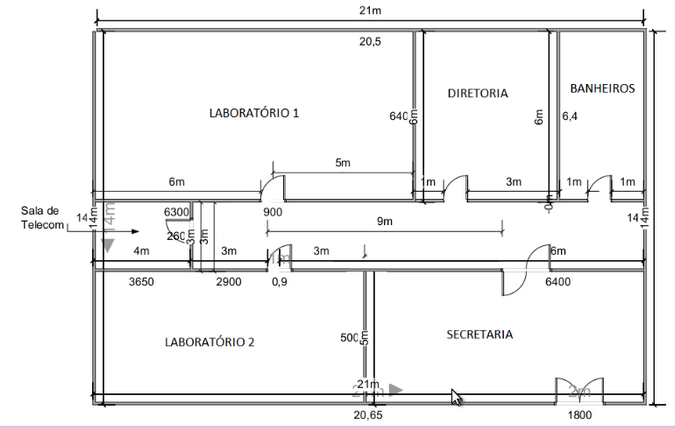
\includegraphics[width=0.8\textwidth]{fig1}
	\caption{Planta baixa}
	\label{fig1}
\end{figure}}

%% ====================================

\section{Topologia Lógica e Definição dos Dispositivos de Rede}
{              
	
\textbf{Iniciando pela necessidade de switch e AP temos os seguintes dados:} 
\begin{itemize}
	\item O escritório será composto por 11 posições, uma Secretaria com 3 posições mais uma sala da       Diretoria com 1 posições, onde em cada ponto de rede que permita conexão física 10/100/1000 Mbps e também a cobertura de sinal wireless no padrão 802.11 b/g/n.;
	\item A escola  contará ainda com duas impressoras de rede, uma mais simples que será posicionada na sala da Diretoria  e outra de maior porte na Secretaria.
	\item É importante que o projeto comporte crescimento de 15% do total de pontos instalados. 
	\item Temos um roteador com Internet e deve sair pelo menos um ponto para LAN.
	\item Um Servidor arquivos e aplicações.
\end{itemize}
	
	
\textbf{Portanto precisamos, em termos de portas de switch, um total de:}

\begin{itemize}
	\item 20 pontos (11 portas para os Laboratórios + 4 portas na secretaria + 2 portas na sala da diretoria + 1 porta para o servidor + 1 porta para o AP + 1 porta para roteador).
	\item Estima um Crescimento de 15% -> (20*15%) = 3  pontos de rede.
	\item Total de portas de switch: 23 portas de rede.
\end{itemize}	
	

Nesse caso temos a opção de um switch de 24 portas. Vamos optar por dois de 16 portas, pois se um “queimar” não irá parar toda a escola.
	
Como teremos o AP com PoE  podemos de esquecer na escolha do modelo do switch um que contemple essa facilidade, além do suporte à criação de VLANs e trunks 802.1Q para conexão com o roteador . As portas do switch devem ser 10/100/1000 Mbps .
	
A especificação para o modelo do AP será 802.11 b/g/n com roteador sem fio com antena omnidirecional de potência maior que a convencional. 
	
O roteador terá no mínimo duas portas para conexão via 10/100/1000 Mbps. Como a Internet será limitada a 10Mbps pode ser uma porta 10/100 Mbps, porém como a LAN será a Giga pois o roteador terá suporte 10/100/1000 Mbps. Como temos uma conexão com a Internet e IP fixo o roteador deverá suportar a configuração de firewall ou então teremos que especificar um firewall para conectar entre a LAN e o roteador. Para esse tipo de topologia vamos escolher um roteador que já faz a parte de firewall e VPN integradas nele.}

\section{Esboço da Topologia Lógica e Definição das VLANs}

Veja na figura a seguir o primeiro esboço do diagrama lógico da rede com os principais dispositivos e suas conexões, onde posicionamos os equipamentos e já definimos as portas dos switches e do roteador onde ficará conectado cada equipamento, podendo assim definir na sequência a alocação de portas para os hosts.


Como foi adotado a separação por VLANs da parte de servidor, AP(roteador Wireless), Sala da Diretoria, Secretaria e Laboratorios 1 e 2, segue a definição de portas por VLAN: 

\begin{itemize}
	\item VLAN 10 – LAB 1: Switch-1 portas 2 a 11 (temos 6 Pcs e deixado mais quatro portas para expansão).
	\item VLAN 20 – DIRETORIA: Switch-1 portas 12 a 16 (temos 1 Pc e 1 impressora e deixado mais três portas para expansão). 
	\item VLAN 30 – WIRELESS: Switch-1 portas 2 gigabit (temos 1 Roteador Wireless). 
	\item VLAN 40 – LAB 2: Switch-2 portas 1 a 9 (temos 5 Pcs  e deixado mais quatro portas para expansão). 
	\item VLAN 50 – SERVIDOR: Switch-2 porta 1 gigabit (temos 1 Servidor).
	\item VLAN 60 – SECRETARIA: Switch-2 portas 10 a 16 (temos 3 Pcs e 1 impressora, deixado mais três portas para expansão).
\end{itemize}
 
 \begin{figure}[H]
 	\centering
 	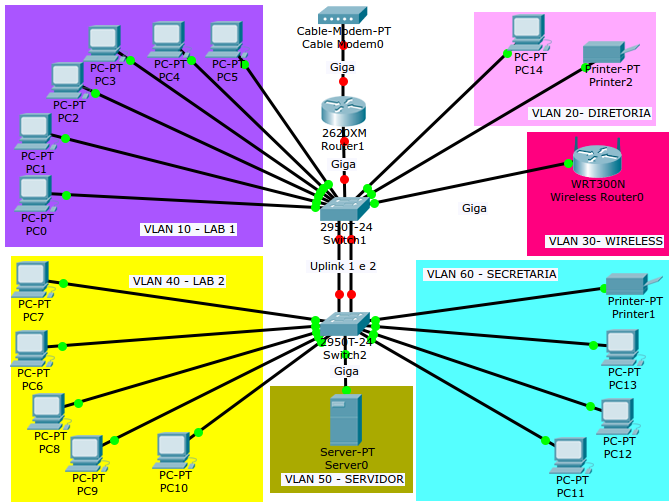
\includegraphics[width=\textwidth]{fig2}
 	\caption{Esboço da Topologia}
 	\label{fig2}
 \end{figure}

A porta 1 do Switch-1, assim como as portas de Uplink 1 e 2 em ambos switches devem ser configuradas como trunk e ter o protocolo 802.1Q e STP habilitados. Apesar de parecer meio estranho, na topologia lógica estarmos definindo que portas dos switches vamos utilizar, pois parece muito mais físico que lógico, pois para a definição das VLANs precisamos desse dado, pois as VLANs são centradas em portas e por isso já definimos nesse passo a alocação de portas por VLAN.

 \begin{figure}[H]
	\centering
	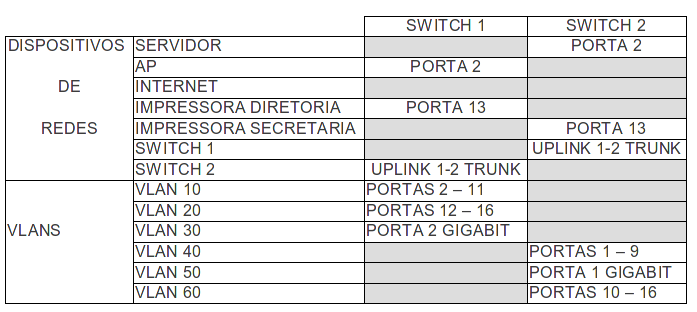
\includegraphics[width=\textwidth]{fig3}
	\caption{Alocação de portas por VLAN}
	\label{fig3}
\end{figure}


\section{Topologia Física}
Nesse projeto será adotado a infraestrutura  centralizada, onde teremos apenas uma sala de telecomunicações/equipamentos facilitando o layout do cabeamento . Se pensarmos nos dois tipos de cabeamento, horizontal e vertical, também é simples deduzir que o cabeamento vertical ficará todo na mesma sala, a não ser o cabo entre o switch-1 e o AP que pode ficar em uma posição diferente dependendo do próximo passo sobre a definição do posicionamento do AP. Todos os demais equipamentos estarão instalados em um mesmo rack  um próximo do outro. 


\subsection{Definição do Posicionamento do AP (Roteador Wireless)}
Para uma maior cobertura da rede sem fio vamos  posicionar o AP no centro do escola e com uma antena de ganho maior que o padrão, por exemplo, uma antena omnidirecional de 12dBi, assim poderemos estimar a quantidade de cabo para a conexão do AP.
\begin{figure}[H]
	\centering
	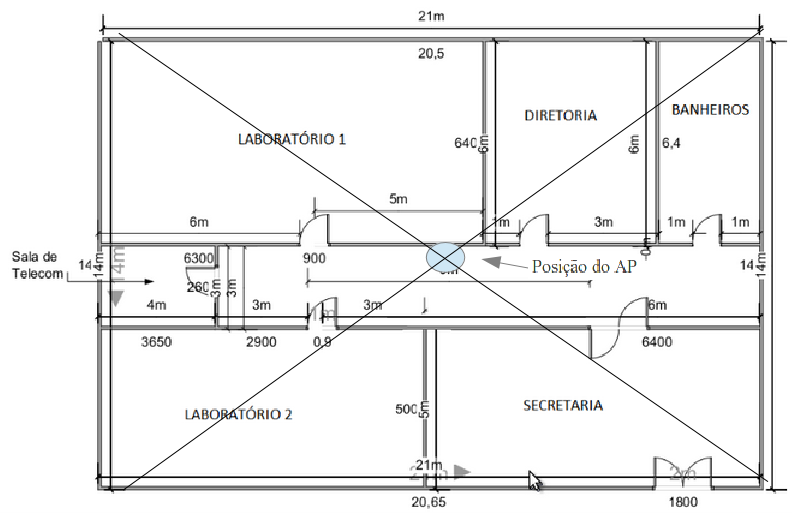
\includegraphics[width=0.8\textwidth]{fig4}
	\caption{Posicionamento do AP}
	\label{fig4}
\end{figure}

\subsection{Definição do rack e seu posicionamento}
 

Como já temos todos os dispositivos de rede que serão utilizados e suas dimensões em Us (Unidades de Rack), podemos agora fazer o dimensionamento de quantos racks iremos precisar. 

Escolhemos a instalação de um  Racks de alumínio com pintura e tratamento anti-corrosivo com 19" de largura (dezenove polegadas ou 483 mm) onde é possível ter uma melhor visualização dos equipamentos e uma melhor dissipação do calor, segue  como cada equipamento será acomodado no rack e a altura de cada um dada em “Us”, conforme listagem abaixo: 
\begin{itemize}
	\item Servidor: 2Us
	\item Equipamentos de Telecom: bandeja e 1U 
	\item Roteador: 1U 
	\item Switch-1: 1U 
	\item Switch-2: 1U 
	\item AP: não será instalado no rack
\end{itemize}
  
Portanto, de equipamentos de rede temos um total de 6Us, porém sem considerar separação entre eles nem os acessórios para o cabeamento como patch panel e passadores de cabo. Sendo assim, vamos finalizar a definição com estes itens, pois temos dois switches de 16 portas, logo, precisaremos de um patch panel de 16 portas e dois passadores de cabo (organizadores de cabo). Vamos utilizar dois patch panels de 16 portas com 2 passadores de cabo, cada um ocupa 1U, portanto teremos mais 4Us, totalizando 10Us. 
Logo, vamos utilizar um rack fechado de piso de 24Us, por exemplo, o qual tem uma altura interna de aproximadamente 1069,2mm (aproximadamente 1m de altura), porém a altura externa será maior devido à estrutura do rack. 
Segue o “Bay-Face” do rack, ou seja, como os equipamentos irão ficar alocados na vista frontal do rack.
\begin{figure}[H]
	\centering
	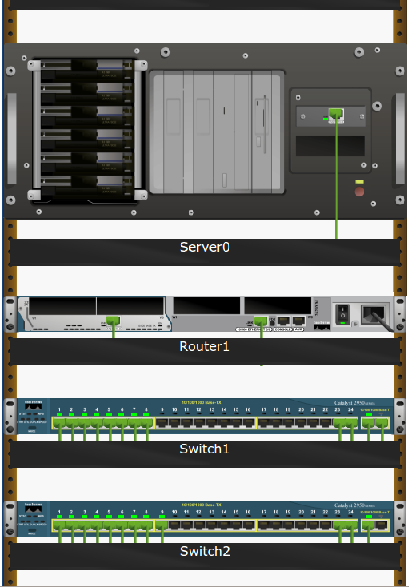
\includegraphics[width=0.5\textwidth]{fig5}
	\caption{Posicionamento dos equipamentos no Rack}
	\label{fig5}
\end{figure}

\begin{figure}[H]
	\centering
	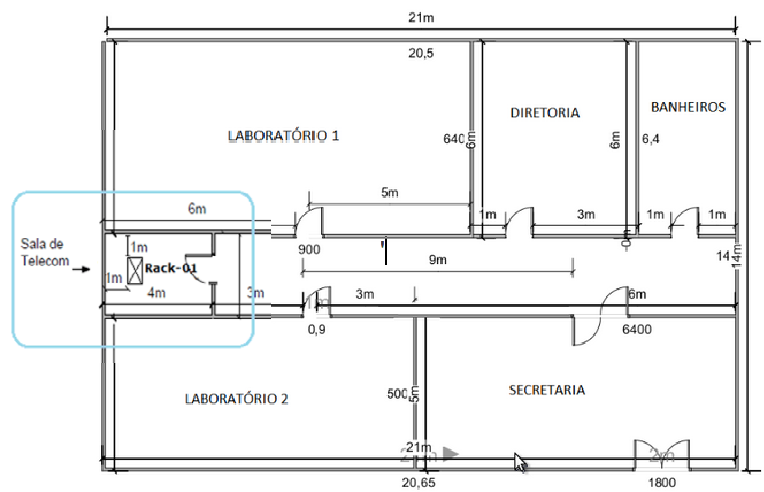
\includegraphics[width=0.8\textwidth]{fig6}
	\caption{Alocação do Rack}
	\label{fig6}
\end{figure}


\section{Dimensionamento dos Cabos}
 
Para dimensionar o cabeamento utilizaremos  as medidas passadas na planta baixa e também a quantidade de computadores por sala para determinar quantos cabos precisaremos em cada lance de cabos para cada uma das salas.  Além disso,  utilizaremos dutos aparentes (canaletas) de parede para a passagem dos cabos da sala de equipamentos/telecomunicações até os pontos de rede que estarão disponíveis nas tomadas de telecomunicações (espelhos). 
Vamos fazer uma estimativa sem considerar subidas e descidas de cabos no início, aí no final colocamos um fator de correção, pois na prática os cabos saem do patch panel do rack, o qual está a uma determinada altura, sai pelo chão até a parede, aí tem mais uma subida para ser distribuído a partir de um duto principal. 

\subsection{Secretaria}
Para a secretaria precisaremos de quatro pontos de rede (3 Computadores e 1  Impressora), portanto vamos traçar o caminho do cabo até a recepção e multiplicar o valor por quatro, pois todos os pontos ficarão na bancada da secretaria . Veja a figura ao lado onde temos do rack até a parede 1m, mais uma subida de 3 metros, mais 4,5m de cabo e mais 13m para chegar ao centro da recepção, para finalizar temos mais 3 metros de descida de cabo, totalizando 24,5m, porém temos 4 pontos na secretaria: 3 Computadores e 1Impressora. Portanto o valor final será de 98 m de cabo.
\begin{figure}[H]
	\centering
	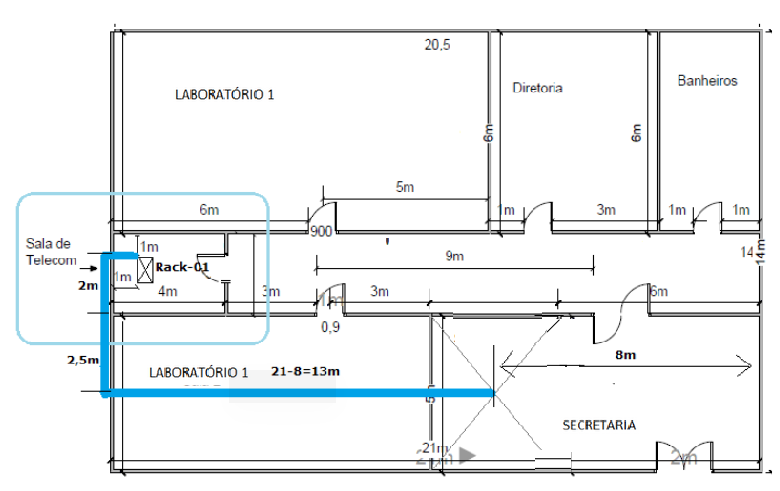
\includegraphics[width=0.8\textwidth]{fig7}
	\caption{Cabeamento do Rack até a Secretaria}
	\label{fig7}
\end{figure}

\subsection{Laboratorio 1}

No laboratorio 1 teremos 6 computadores, portanto vamos ter 1m da saída do rack até a parede, mais uma subida de 3 metros, 7 metros até o final da parede, mais 12 metros, mais 6 metros para a parede frontal, mais 2,5m até a metade da parede até a porta e 3 metros de descida de cabo, portanto termos um total por cabo de 34,50m de cabo, porém temos que multiplicar por 6 (6 micros), totalizando 207m de cabo.
\begin{figure}[H]
	\centering
	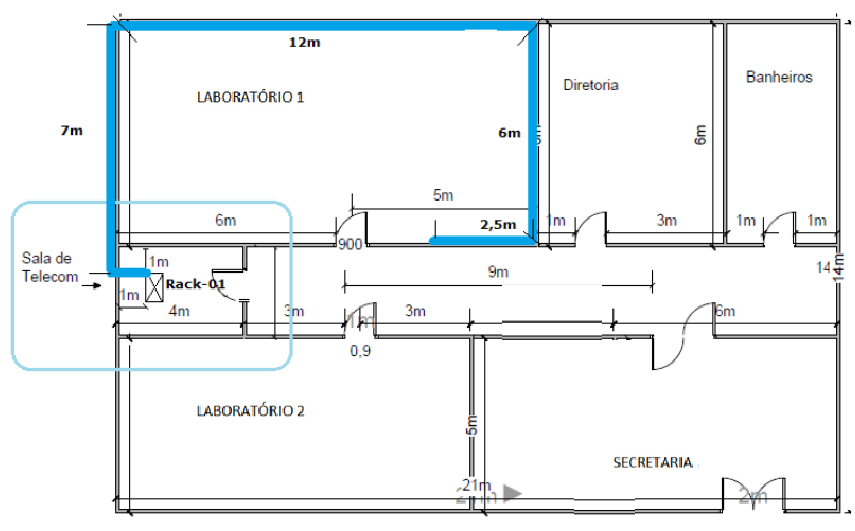
\includegraphics[width=0.8\textwidth]{fig8}
	\caption{Cabeamento do Rack até o Laboratório 1}
	\label{fig8}
\end{figure}

\subsection{Laboratorio 2}

No laboratorio 2 teremos 5 computadores, portanto vamos ter 1 metro de cabo do rack até a parede, 7 metros até a ponta da outra parede, 11 metros, mais 5 metros e 1,5m até metade da parede onde temos a porta, mais 3 metros de subida no rack e 3 metros de descida na sala, totalizando 31,50m por cabo, porém temos um total de 5 computadores o que dará 157,50m de cabo.
\begin{figure}[H]
	\centering
	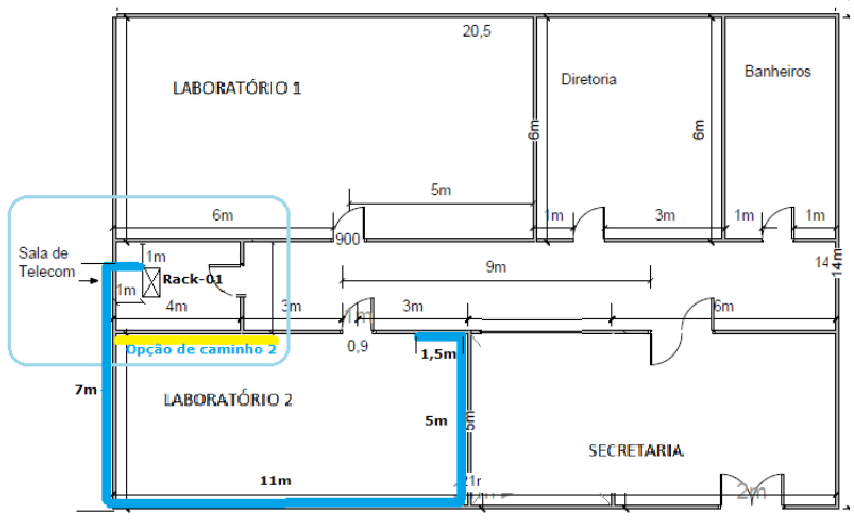
\includegraphics[width=0.8\textwidth]{fig9}
	\caption{Cabeamento do Rack até o Laboratório 2}
	\label{fig9}
\end{figure}


\subsection{Diretoria}
Na Sala da diretoriatemos 1 computador e 1 impressora, portanto teremos 1m do rack até a parede, mais 7 metros até o final da parede, mais 7 metros até o final da parede da diretoria, mais 6 m para chegar à parede da porta e 1,5m para chegar até a metade da parede da porta.Além disso, temos 3m de subida no rack e 3m de descida na sala da diretoria. Portanto teremos 32,50m por cabo, porém como temos dois pontos de rede o total será de 65m de cabo.
\begin{figure}[H]
	\centering
	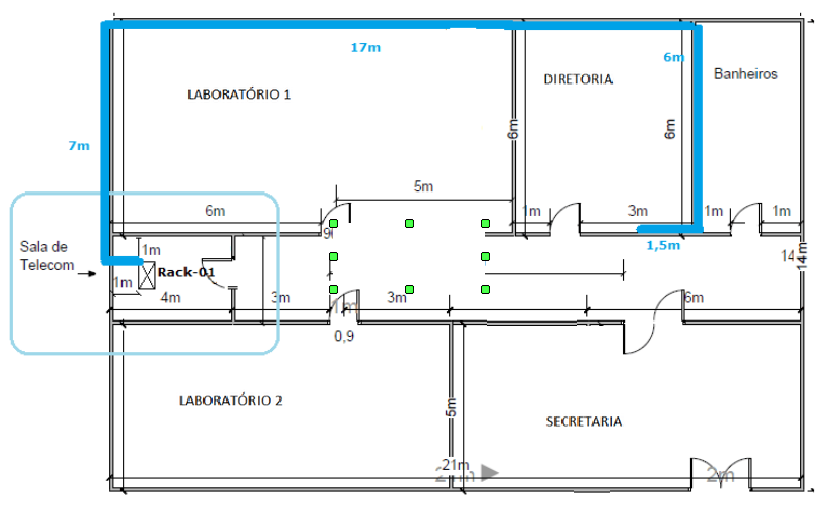
\includegraphics[width=0.8\textwidth]{fig10}
	\caption{Cabeamento do Rack até a Diretoria}
	\label{fig10}
\end{figure}

\subsection{Access Point}
Agora ainda está faltando o AP que ficará centralizado e fixado no teto do corredor próximo a sala de Diretoria, portanto temos mais uma subida de cabo para considerar. portante teremos um total de 1m até a parede, mais uma subida de 3m, mais 1 metro até a prumada da parede lateral, 11m até chegar ao centro da edificação, mais 1 metro até o AP e vamos colocar mais 1m de folga de cabo, pois o AP ficará fixado no teto, totalizando 18m de cabo.
\begin{figure}[H]
	\centering
	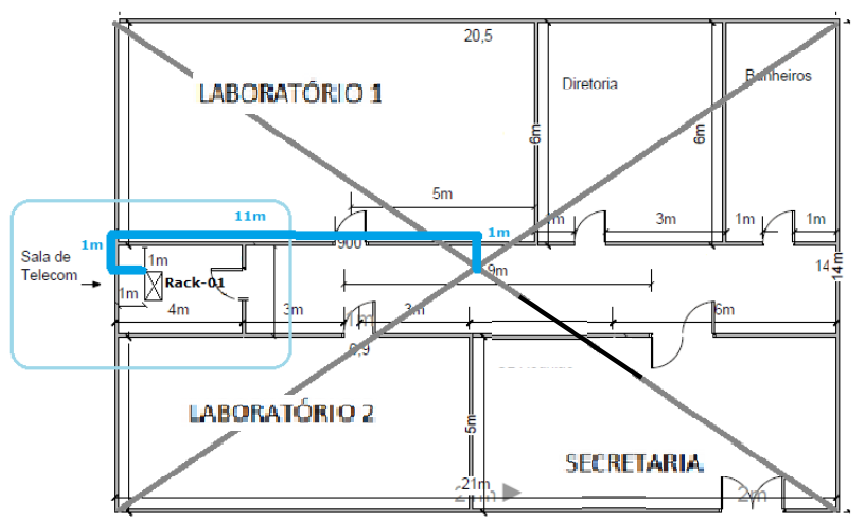
\includegraphics[width=0.8\textwidth]{fig11}
	\caption{Cabeamento do Rack até o AP}
	\label{fig11}
\end{figure}

\section{Plano de certificação}
Os testes de certificação são descritos na norma ANSI/TIA/EIA-568B e será executado em toda rede seguindo as etapas abaixo:
\begin{itemize}
		
		\item MAPA DE FIOS- Efetua o mapeamento da pinagem entre os condutores e indica falhas de
		contatos elétricos, pares trocados etc.
		\item ATENUAÇÃO- Mede as perdas nas transmissões de sinais causadas por cabos de categoria
		inferior, comprimento excessivo e conexões mal feitas.
		\item COMPRIMENTO DO CABO- Indica o comprimento do cabo pela técnica TDR (Time Domain
		Reflectometer), reflectometria no domínio do tempo, cujo funcionamento básico consiste na injeção
		de um pulso elétrico em uma extremidade do cabo e a cronometragem do tempo de retorno do
		pulso injetado e refletido na mesma extremidade do cabo. O trecho fixo, com cabo rígido está
		limitado a 90,0m; ou 100,0m incluindo os dois patch cord's.
		\item NEXT- Mede erros causados por fontes externas tais como no-breaks, lâmpadas fluorescentes,
		máquinas de xerox; qualidade dos acessórios como patch panel, tomadas, ferramentas punch
		down de crimpagem etc.
		\item ELFEXT- Mede parâmetros com aplicações em gigabit, com os quatro pares energizados ao
		mesmo tempo.
		\item RESISTÊNCIA - Indica a resistência do cabo para corrente contínua em determinado lance.
		\item IMPEDÂNCIA- Mede a impedância do cabo em diversas frequências estabelecidas pela norma. A
		impedância fora dos padrões implica em grande atenuação do sinal. É causada normalmente por
		tração excessiva e torcimento dos condutores.
		\item CAPACITÂNCIA- Mede erros por capacitância, causado por ruído excessivo no cabo, blindagem
		interrompida etc.
		\item PERDA DE RETORNO-Mede o percentual do sinal emitido que, indevidamente, retorna para a
		fonte.
		\item ATRASO DE PROPAGAÇÃO- Mede o tempo de propagação do sinal comparando-o com o tempo
		limite estabelecido pela norma.
		\item ACR- Mede os erros de ACR, causados por categoria dos acessórios errada, conexões mal feitas,
		cordões de manobra não flexíveis etc.
		Outros testes como: Área de Margem, Power Sum ACR, Power Sum ELFEXT e Power Sum NEXT,
		são complementares. Normalmente, não significa erro quando os principais testes estão corretos.
		Além dos valores medidos, o relatório deverá conter os limites estabelecidos, a margem de erro e a
		faixa de frequência utilizada; sendo esta de 1 a 250MHZ, para CAT-6.	 
\end{itemize} 

\section{Plano de manutenção}

Uma vez instaladas, as redes necessitam de manutenções periódicas, preventivas e/ou corretivas. Assegurando o melhor funcionamento dos elementos da rede através de relatórios e acompanhamento de cada ativo da rede, para tal projeto recomendamos um plano de Manutenção Preventiva que contará com a visita mensal pré-agendada de um técnico qualificado, onde ele verificará as condições de hardware e software dos equipamentos, além de serviço de gerencimento da rede de computadores, presencial e através de conexão remota, serviço de backup e outros.

\subsection{Plano de expansão}
Conforme citado acima, temos 15 porcento de capacidade de expansão, mas como optamos pela utilização de dois Switches de 16 portas cada e utilizamos apenas 20 portas nos restam 12 portas para serem utilizada caso necessite expandir a rede sem utilização de outro dispositivo de camada 2, caso houver a necessidade de expansão com um volume acima do que restou, o layout possibilita a instalação de mais um Switch na camada 2 com a quantidade de portas que for necessária para atender a demanda. 



\section{Orçamento}
Segue orçamento para realização do projeto:
\begin{figure}[H]
	\centering
	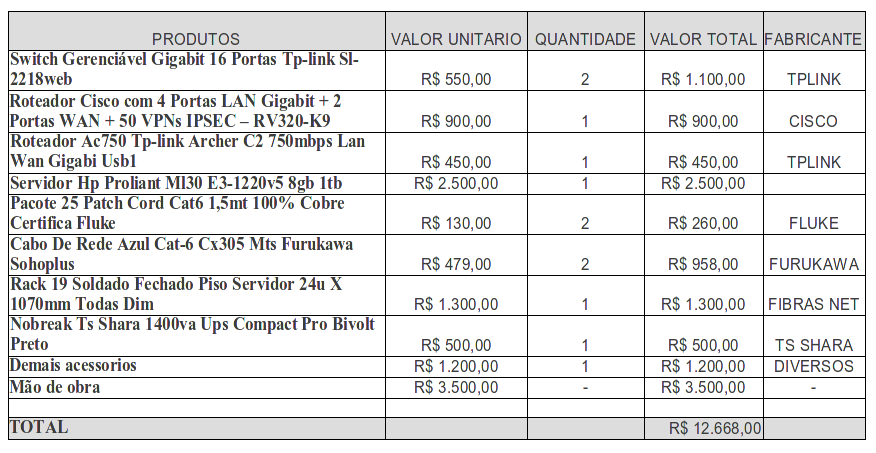
\includegraphics[width=\textwidth]{fig12}
	\caption{Orçamento}
	\label{fig12}
\end{figure}

\section{Cronograma}
O cronograma abaixo apresentado serão os dias para implantação e reestruturação.
\begin{itemize}
	\item Reunião – 3 dias
	\item Planejamento – 5 dias
	\item Desenvolvimento do cronograma e apresentação – 5 dias
	\item Distribuição de tarefas – 3 dias
	\item Implementação – 4 dias
	\item Implantação – 8 dias
	\item Treinamento – 2 dias
\end{itemize}



\section{Referências bibliográficas}
\begin{itemize}
	\item  Paulo Sérgio Marin - Cabeamento Estruturado - Desvendando Cada Passo - Do Projeto à Instalação - 5ª Edição 2013 Ed. Érica
	\item http://www.tp-link.com.br/products/details/cat-40TL-SL2218.html
	\item http://www.tp-link.com.br/products/details/cat-9Archer-C2.html 
	\item https://www.fourserv.com.br/roteador-cisco-dual-wan-4-portas-4x-lan-gigabit-2x-wan-50-vpns-ipsec-mpn-rv320-k9-na
	\item https://www.bztech.com.br/hp/servidor-proliant-ml30-g9
\end{itemize}  


%% ***********************************************************************
%% === ate aqui    =====  ================================================
%% ***********************************************************************
\end{document}